\documentclass[11pt,a4paper]{article}

\usepackage[utf8]{inputenc}
\usepackage[T1]{fontenc}
\usepackage{lmodern}
\usepackage{amsmath, amssymb}
\usepackage{graphicx}
\usepackage{geometry}
\usepackage{booktabs}
\usepackage{array}
\usepackage{microtype}
\usepackage{setspace}
\usepackage{xcolor}
\usepackage{cite}
\usepackage[colorlinks=true,linkcolor=blue!55!black,citecolor=blue!55!black,urlcolor=blue!55!black,pdftitle={Independent Formal Verification, Epistemic Spine Cartography, and Comparative Auditing of Riemann Hypothesis Proof Claims},pdfauthor={Manuel Menendez-Gonzalez}]{hyperref}

\geometry{margin=0.82in}
\setstretch{1.11}
\setlength{\emergencystretch}{3em}
\pagestyle{plain}
\newcommand{\code}[1]{\texttt{\small #1}}

% --- DETERMINISTIC FLOAT PLACEMENT & SECTION-BARRIER ENGINE ---
\renewcommand{\topfraction}{0.95}
\renewcommand{\bottomfraction}{0.95}
\renewcommand{\textfraction}{0.04}
\renewcommand{\floatpagefraction}{0.85}
\setcounter{topnumber}{4}
\setcounter{bottomnumber}{4}
\setcounter{totalnumber}{6}
\setlength{\textfloatsep}{10pt plus 2pt minus 2pt}
\setlength{\floatsep}{8pt plus 2pt minus 2pt}
\setlength{\intextsep}{10pt plus 2pt minus 2pt}
\makeatletter
\providecommand{\FloatBarrier}{%
  \par
  \expandafter\ifx\csname @freelist\endcsname\relax\else
    \ifx\@deferlist\@empty\else
      \clearpage
    \fi
  \fi
}
\let\orig@section\section
\renewcommand{\section}{\FloatBarrier\orig@section}
\makeatother

% --- METADATA ---
\title{\textbf{Independent Formal Verification, Epistemic Spine Cartography, and Comparative Auditing of Riemann Hypothesis Proof Claims}}

\author{Manuel Men{\'e}ndez-Gonz{\'a}lez\thanks{Corresponding author: \texttt{menendezgmanuel@uniovi.es}. ORCID: \texttt{0000-0002-1825-0097}. Public Verification Dossier (v1.1): \url{https://github.com/Fundacion-de-Neurociencias/riemann-hypothesis-audit-dossier}.}}

\date{November 24, 2026 $\cdot$ Preprint Version 1.1.1}

\begin{document}

\maketitle
\thispagestyle{plain}

\begin{abstract}
\noindent We report an independent computational verification, transitive fresh-environment kernel replay, cryptographic provenance audit, deductive dependency cartography, human-comprehensible verification anatomy, and comparative manuscript evaluation of two contemporary claims addressing the Riemann Hypothesis (RH) and Generalized Riemann Hypothesis (GRH): (i) Levent Alp{\"o}ge's AI-assisted Lean~4 formalization comprising 175,187 modules (17,374,215 lines), and (ii) Alessandro Maria Masullo's 940-page informal human manuscript. Compiled from source on an independent Apple M4 Max workstation (16-core ARM64, 64\,GB unified memory) under Lean~\texttt{v4.33.1}, \texttt{lake build} completed deterministically with clean exit status in 127,812\,seconds ($\approx$35.5\,hours), producing 183,889 \texttt{.olean} binary artifacts (98\,GB build footprint). Subsequent transitive fresh-environment replay via \texttt{lake env leanchecker -{}-fresh} completed independently in 26,898\,seconds (7\,h 28\,min 18\,s, zero exit status), ruling out binary corruption, environment manipulation, and metaprogramming bypasses across all imported and exported declarations. Axiom tracing (\texttt{\#print axioms}) over all five exported root theorems---anchored cleanly in canonical \texttt{Mathlib} definitions (\texttt{RiemannHypothesis} and \texttt{DirichletCharacter.LFunction}) across a human-readable external statement specification of only 28~lines (specification-to-proof ratio $1.62 \times 10^{-6}$)---confirmed zero \texttt{sorry} placeholders, zero custom axioms, and exclusive reliance on \texttt{[propext, Classical.choice, Quot.sound]}. Conversely, forensic segmentation of the 940-page informal draft uncovered a blocking deductive gap in Chapter~13 (stub sections~13.1--13.2 and an empty conclusive Theorem~13.3.1.2), alongside 19 unresolved cross-references and 10 draft placeholders. Graph-theoretic dependency analysis across the 818,755 formal theorems and lemmas locates the structural bottleneck at deductive depths~6--7 within the toroidal uniformization interface of the reciprocity layer (fan-in 2,390, 2,379 cross-layer shortcut arcs) and identifies six recurring algebraic-arithmetic engines led by Galois modularity patching (109,260 modules) and iterated unitary theta-lift chains (15,750 modules). Beyond computational certification, we translate both what RH signifies---optimal deterministic cancellation rooted in combinatorial necessity rather than randomness or physical fine-tuning, contrasting unbounded arithmetic law against finite physical instantiation bounds---and how formal verification itself guarantees trust. Interpreting both artifacts through the Epistemia framework~\cite{quattrociocchi2025}, Thurston's distinction between verification and understanding~\cite{thurston1994}, and resource-rational cognitive science~\cite{griffiths2026}, we show why machine-checked validity (Epistemia risk 0.245, machine-verified yet human-opaque) and human comprehension decouple orthogonally. Finally, we demonstrate how our local 64\,GB workstation hit a 46.47\,GB virtual-memory wall during monolithic flat serialization ($\sim$61.57\,GB full export required by clean-room external kernels), bypassed that ceiling via memory-bounded module-by-module \texttt{.olean} replay with \texttt{lean4lean}~\cite{carneiro2026} (achieving 28,357 / 175,187 modules and 616,173 declarations checked with 0 failures---including local reproduction of all five elevated-fuel kernel-decision modules---actively streaming toward full archive closure), and distill four generalizable engineering safeguards for autonomous scientific auditing systems.
\end{abstract}

\section{Introduction}

On November 20, 2026, mathematics witnessed an acute epistemic divergence. Levent Alp{\"o}ge publicly released a compressed Lean~4 codebase~\cite{alpoge2026} asserting unconditional formal proofs of the Riemann Hypothesis and the Generalized Riemann Hypothesis for Dirichlet $L$-functions developed iteratively with Claude, accompanied by a four-page note acknowledging that unfiltered prose expansion exceeded 250,000 pages. On the same day, Ravi Vakil posted a hurried announcement of Alessandro Maria Masullo's twelve-year, 940-page human \LaTeX{} manuscript proposing a spectral trace-formula proof of GRH for general Hecke $L$-functions~\cite{vakil2026}.

This juxtaposition crystallizes a central metascientific challenge articulated by Quattrociocchi, Capraro, and Perc~\cite{quattrociocchi2025} and grounded computationally by Griffiths~\cite{griffiths2026}: classical mathematical peer review implicitly assumes that \emph{deductive validity} and \emph{human surveyability} move together. A 17.37-million-line formal corpus shatters that assumption. Addressing it requires more than returning a binary compiler exit code; it demands a dual scientific contribution:
\begin{enumerate}
  \item \textbf{Rigorous Multi-Stage Auditing:} Independently certifying cryptographic provenance, static soundness, statement fidelity, reference-kernel compilation, transitive fresh replay, and informal manuscript completeness under transparent resource boundaries.
  \item \textbf{Cognitive and Conceptual Translation:} Making intelligible to mathematicians, scientists, and philosophers \emph{what} the Riemann Hypothesis signifies, \emph{how} formal verification certifies truth without requiring human inspection of millions of lines, \emph{how} the proof's core algebraic machinery works, and \emph{why} formal certification marks the beginning---not the end---of human understanding.
\end{enumerate}

\section{What the Riemann Hypothesis Means: Deterministic Cancellation and Combinatorial Necessity}

Before auditing seventeen million lines of formal code, clarity requires dispelling two persistent misconceptions surrounding the Riemann Hypothesis: that RH asserts ``perfect randomness'' among prime numbers, or that its validity reflects a delicate physical or metaphysical calibration of the cosmos.

\subsection{Optimal Deterministic Cancellation Versus Apparent Randomness}

The prime numbers contain no randomness whatsoever: they are uniquely fixed the instant addition (unit stepping, $+1$) and multiplication (packing units into equal-sized blocks) are defined over the integers $\mathbb{Z}$. Regardless of linguistic notation or numerical base, placing two identical discrete units side by side produces a tessellable, composite configuration; by sheer combinatorial necessity, the boundary between decomposable packings and irreducible primes emerges automatically once discrete multiplicity exists.

What the Riemann Hypothesis asserts---by confining all non-trivial zeros $\rho$ of $\zeta(s)$ (and analogously of Dirichlet $L$-functions $L(s,\chi)$ under GRH) to the critical line $\operatorname{Re}(s) = \tfrac{1}{2}$---is \textbf{optimal deterministic cancellation} across that additive--multiplicative boundary. By Helge von Koch's classical equivalence~\cite{vonkoch1901}, RH is equivalent to the sharp error bound on the prime counting function $\pi(x)$ relative to the logarithmic integral $\operatorname{Li}(x)$:
\begin{equation}
  \pi(x) = \operatorname{Li}(x) + O\!\left(\sqrt{x}\log x\right).
\end{equation}
Because square-root fluctuation scales mirror the deviation of an unbiased random walk, RH is frequently popularized as stating that primes behave ``as randomly as coin flips.'' That analogy fails in two decisive respects:
\begin{enumerate}
  \item \textbf{Absence of Macroscopic Oscillatory Bias:} Through the Riemann--von Mangoldt explicit formula, every non-trivial zero $\rho = \beta + i\gamma$ contributes an oscillatory term of amplitude $\sim x^{\beta}$ to prime counts. Even a \emph{single} zero with $\beta > \tfrac{1}{2}$ would inject a persistent macroscopic wave creating vast prime-poor deserts followed by anomalous local accumulations.
  \item \textbf{Rigid Spectral Repulsion Rather Than Independence:} The spacings between consecutive zeta zeros do \emph{not} behave like independent Poisson random points. As conjectured by Montgomery~\cite{montgomery1973} and corroborated numerically across millions of zeros by Odlyzko~\cite{odlyzko1987}, normalized zero spacings exhibit strong \textbf{level repulsion} matching the eigenvalues of random Hermitian matrices in the Gaussian Unitary Ensemble (GUE).
\end{enumerate}
Thus, RH describes not miraculously tuned chance, but a completely deterministic arithmetic structure whose internal rigidity forbids large-scale bias between additive stepping and multiplicative packing.

\subsection{Bounded Physical Instantiation Versus Unbounded Arithmetic Law}

A natural philosophical question follows: if the observable universe is finite, does an asymptotic statement reaching to infinity carry physical meaning? Answering clearly requires separating two distinct ontological planes:
\begin{itemize}
  \item \textbf{The Unbounded Law of Formal Operations (the Medium):} Arithmetic operations ($+, \times, -, \div$) are unbounded by definition---logically, one can always add $+1$ upward or subdivide further downward. Within this formal domain, the combinatorial grammar governing primes and composites is completely immutable, independent of contingent physical constants ($G$, $\hbar$, $c$).
  \item \textbf{The Bounded Window of Physical Instantiation (the Vessel):} Physical reality instantiates only a finite slice of those operations delimited by hard empirical cutoffs: a lower spatial granularity floor near the Planck scale ($l_P \approx 1.616 \times 10^{-35}\,\mathrm{m}$) and an upper information-processing ceiling. Over its history, the observable universe can have performed at most $\sim 10^{120}$ elementary logic operations on $\sim 10^{90}$ bits of matter and radiation~\cite{lloyd2002}, while its total cosmic event horizon entropy is bounded around $S_{\mathrm{CEH}} \approx 2.6 \times 10^{122}\,k_B$~\cite{bekenstein1981,egan2010}. Beyond those cutoffs, iterating $+1$ ceases to correspond to physically instantiated states and becomes pure symbolic structure.
\end{itemize}

From a strictly physicalist standpoint, numerical verification has already confirmed RH up to height $T = 3 \times 10^{12}$~\cite{platt2021}; an off-line zero emerging only at some astronomical scale such as $10^{10^{500}}$ would lie forever outside the causal and computational capacity of the cosmos. Yet arithmetic provides a celebrated demonstration of why mathematicians cannot rest with finite verification inside the physical vessel: for more than a century, every computation ever performed supported $\pi(x) < \operatorname{li}(x)$. Nevertheless, Littlewood~\cite{littlewood1914} proved that $\pi(x) - \operatorname{li}(x)$ reverses sign infinitely often, with modern explicit bounds placing the first crossover below $e^{727.95134} \approx 1.397 \times 10^{316}$~\cite{saouter2015}---vastly exceeding the $\sim 10^{80}$ baryons or $\sim 10^{122}$ horizon bits of the observable universe. No physical computer bounded by cosmic entropy could ever have witnessed that sign change by brute enumeration, yet the inversion was already inscribed in the laws of arithmetic.

This delineates a clean division of labor: \textbf{physics characterizes the finite vessel} between empirical cutoffs, whereas \textbf{mathematics characterizes the intrinsic law of the medium}, distinguishing scale-invariant structural invariants from finite-scale mirages. Confirming RH changes nothing causally inside physical bounds, yet certifies that the cancellation observed inside our computational horizon is a \textbf{necessary structural consequence} of arithmetic---rendering teleological or physicalist ``fine-tuning'' interpretations unnecessary. Given the axioms of addition and multiplication, any off-line zero entails a logical contradiction.

\section{Making Machine Verification Intelligible: Anatomy of Formal Trust and Static Audit}

When a proof spans 17.37 million lines, human readers naturally ask an operational question: \emph{how can we trust a computer check we cannot read line by line, and how might a claimed formal proof deceive us?}

\subsection{Anatomy of Formal Trust: How a Machine Proof Could Fail}

The decisive epistemic leverage of a dependent-type proof assistant like Lean~4 rests on \textbf{asymmetric auditing}: a human does \emph{not} need to verify millions of proof steps to know \emph{what} was proved, provided four distinct failure vectors are audited systematically (\textbf{Table~\ref{tab:trust_anatomy}}).

\begin{table}[!htb]
\centering
\caption{Anatomy of formal trust: four failure modes by which a machine-checked proof claim can mislead, what humans must inspect directly, and what our independent verification establishes.}
\label{tab:trust_anatomy}
\footnotesize
\setlength{\tabcolsep}{4pt}
\begin{tabular}{@{}>{\raggedright\arraybackslash}p{0.18\textwidth}>{\raggedright\arraybackslash}p{0.27\textwidth}>{\raggedright\arraybackslash}p{0.19\textwidth}>{\raggedright\arraybackslash}p{0.31\textwidth}@{}}
\toprule
\textbf{Failure Vector} & \textbf{How a Claim Could Mislead} & \textbf{What Humans Must Read} & \textbf{Verification Outcome (v1.1)} \\
\midrule
\textbf{1. Specification / Statement Hacking} & Proving a weakened, shadowed, or vacuous theorem (e.g., redefining the $L$-function locally, omitting domain guards, or exploiting Lean's total division \texttt{x / 0 = 0}). & Only the \textbf{28-line external specification} (root statement and export files) plus standard \texttt{Mathlib} symbols. & \textbf{Cleared:} Exact semantic match verified with 0 shadowing hazards; specification-to-proof ratio $1.62 \times 10^{-6}$. \\
\addlinespace[4pt]
\textbf{2. Proof Skipping or Axiom Smuggling} & Leaving unfinished holes (\texttt{sorry}), custom \texttt{axiom}s, unverified compiled code (\texttt{native\_decide}, \texttt{@[implemented\_by]}), or environment mutations. & Static audit summary + verbatim \texttt{\#print axioms} output. & \textbf{Cleared:} 0 holes, 0 custom axioms, 0 unsafe bypasses across 175,187 modules; strictly \texttt{[propext, Classical.choice, Quot.sound]}. \\
\addlinespace[4pt]
\textbf{3. Verifier Bug or Binary Tampering} & Soundness bug in Lean \texttt{v4.33.1} kernel or corrupted/manipulated \texttt{.olean} environment state. & Kernel replay logs and external checker reports. & \textbf{Lean \texttt{v4.33.1} Cleared / Bounded \texttt{lean4lean} Streaming:} Full build (127,812\,s) + \texttt{leanchecker -{}-fresh} (26,898\,s, clean exit); bounded-RAM \texttt{lean4lean} cleared 28,357 / 175,187 modules (616,173 decls, 0 failures, all 5 elevated-fuel modules); monolithic 61.57\,GB clean-room flat export stalled at 46.47\,GB on 64\,GB RAM (Sec.~\ref{sec:boundaries}). \\
\addlinespace[4pt]
\textbf{4. Prose Scope Inflation} & Claiming broader theorems in prose (e.g., Extended RH) than compiled in Lean. & Comparison between accompanying prose note and formal root statements. & \textbf{Flagged:} RH and Dirichlet GRH compiled (machine-verified, human-opaque, risk 0.245); ERH extrapolation suspends judgment (risk 0.4075). \\
\bottomrule
\end{tabular}
\end{table}

\subsection{Bit-Exact Input Pinning}

Every primary source artifact was retrieved from public origins and verified locally by SHA-256 checksum:
\begin{itemize}
  \item \textbf{Formal Archive (\texttt{alpo.ge/}):} 239,275,554 bytes, SHA-256 \code{9631b4f020199e58\allowbreak 0ba86178cb56c6e9\allowbreak b09f690c2369a80d\allowbreak c4334aa93f49c7fc}, bit-identical against the public mirror \url{https://github.com/jsmorph/rh}.
  \item \textbf{Accompanying Explanatory Note:} 245,114 bytes, SHA-256 \code{3fc97784b71ddd44\allowbreak ff8aa0a177e99622\allowbreak a1c61b13cfa843a0\allowbreak 989ee4a7a0cfeb8d}.
  \item \textbf{Root Specification and Export Modules:} 16-line statement file (SHA-256 \code{79ef7ca776e42abe\allowbreak 1f46caee13ea09bd\allowbreak 19f1e2d0b1620d8d\allowbreak 5d200258f33b47bf}) and 12-line export file (SHA-256 \code{017645ca448f2fd1\allowbreak f6fd5c4c2cb2c6e9\allowbreak 6e472725be13f6e1\allowbreak 80ca6e1574360939}), verified identical between tarball and build workspace.
  \item \textbf{Pinned Environment:} \texttt{leanprover/lean4:v4.33.1} with \texttt{Mathlib} revision \code{0df444a360eaa60a\allowbreak b8c11dca51a86af6\allowbreak 92955474}.
  \item \textbf{Informal Draft (\emph{The Music of the Primes}):} 6,756,996 bytes (940 pages, compiled with \texttt{pdfTeX-1.40.25}), SHA-256 \code{e039d3f6cf0a4b14\allowbreak f03c7edb85097752\allowbreak dd65c0a2fe543c76\allowbreak fe992be234f97bf}.
\end{itemize}

\subsection{Full-Archive Static Soundness Inventory}

Exhaustive streaming lexical analysis across all 175,190 archive files (175,187 \texttt{.lean} sources totaling 17,374,215 lines and 1,030,531,854 bytes) recorded:
\begin{itemize}
  \item 784,092 \texttt{theorem} declarations, 34,663 \texttt{lemma} declarations (818,755 total), 212,819 \texttt{def}, 13,202 \texttt{abbrev}, 8,286 \texttt{structure}, 4,581 \texttt{instance}, 121 \texttt{inductive}, and 43 \texttt{class} declarations.
  \item \textbf{0} missing local imports across the full Unicode module graph, with 174,767 \texttt{.lean} files (99.76\%, 17,330,139 lines) statically reachable from the root export module and only 420 pruned deadweight files (0.24\%).
  \item \textbf{0} custom \texttt{axiom}, \texttt{sorry}/\texttt{sorryAx}/\texttt{admit}, \texttt{native\_decide}, \texttt{unsafe}, \texttt{@[implemented\_by]}, \texttt{@[extern]}, \texttt{@[csimp]}, \texttt{opaque}, or kernel-bypass declarations.
  \item Five environment-modification calls in build-aid modules alter only tactic search-suggestion denylists (logically inert), and three metaprogramming helpers invoke kernel-checked declaration additions. Two \texttt{partial def} declarations exist exclusively inside metaprogramming helpers, never within mathematical theorem objects.
\end{itemize}

\subsection{Statement Fidelity and Trusted Computing Base Ratio}

Auditing \emph{what} was proved---independently of the internal tactics that prove it---concentrates in a 28-line external specification comprising the public statement definitions and root theorem exports. Relative to the 17,330,139 lines of active formal code reachable from the root, this yields a trusted specification ratio of $1.62 \times 10^{-6}$. Because Lean~4 defines arithmetic operations such as division and inversion as total functions (for instance, returning $0$ on division by zero), a critical check is whether any root or intermediate theorem becomes vacuously true through unguarded denominators or degenerate prime-power bases. Inspection confirms zero unguarded total-function hazards in the 28-line public specification; throughout the intermediate critical-line and strip modules, inverses operate strictly on character-group elements and prime-power bases guarded by explicit primality hypotheses, never via unguarded field division.

Semantic comparison against canonical \texttt{Mathlib} predicates confirms exact fidelity for both the critical-line and right-half-plane non-vanishing theorems for Dirichlet $L$-functions (\texttt{DirichletCharacter.LFunction}). Furthermore, \texttt{Mathlib}'s \texttt{RiemannHypothesis} predicate quantifies over all zeros in $\mathbb{C} \setminus \{1, -2, -4, \dots\}$---a formulation strictly stronger as a standalone statement than restricting to the critical strip $0 < \operatorname{Re}(s) < 1$, and classically equivalent via the functional equation and non-vanishing on $\operatorname{Re}(s) \ge 1$ established in the strip-reduction modules. Finally, although two auxiliary $L$-function definitions appear inside isolated local namespaces for local zeta and Hecke constructions, neither shadows or alters \texttt{DirichletCharacter.LFunction} in the exported theorem statements.

\section{Independent Compilation, Metamathematical Axiom Reading, and Resource Boundaries}

\subsection{Reference Hardware Compilation and Transitive Fresh Replay}

Clean compilation and transitive replay were executed independently on an \textbf{Apple M4 Max (16-core ARM64, 64\,GB unified memory, macOS Darwin 25.5.0)} under \texttt{leanprover/lean4:v4.33.1} (\textbf{Figure~\ref{fig:verif_epistemia}A}):
\begin{itemize}
  \item \textbf{Root Specification Compilation:} Completed with zero exit status in 31\,seconds.
  \item \textbf{Full Library Build (\texttt{lake build}):} Completed with zero exit status in \textbf{127,812\,seconds} (35\,h 30\,min 12\,s), compiling 175,187/175,187 project modules (183,889 \texttt{.olean} files total including cached \texttt{Mathlib} units; 98\,GB build directory footprint).
  \item \textbf{Axiom-Trace Verification (\texttt{\#print axioms}, 110\,seconds, zero exit status):} Archived in the public verification dossier (SHA-256 \code{590d5252e7e5a4e6\allowbreak d9faef1895216c77\allowbreak eb103d6667037d83\allowbreak 2eaedaa34fa3186d}). All five exported root theorems---the Riemann Hypothesis, critical-line location of $\zeta(s)$ zeros, and three Dirichlet $L$-function non-vanishing and critical-line theorems (including primitive characters)---depend strictly on:
  \begin{center}
    \texttt{[propext, Classical.choice, Quot.sound]}
  \end{center}
  \item \textbf{Transitive Fresh-Environment Replay (26,898\,seconds / 7\,h 28\,min 18\,s, zero exit status):} Executed via \texttt{lake env leanchecker -{}-fresh} (2026-11-23T06:35:06Z $\to$ 2026-11-23T14:03:24Z) and archived in the public dossier (SHA-256 \code{ff8ea3d0b4db9f21\allowbreak f2a09513a5b20c1d\allowbreak 2d6d106566030aa7\allowbreak f21e50156966f95c}), independently re-elaborating every imported and exported declaration starting from an empty kernel environment.
\end{itemize}

\begin{figure}[!htb]
  \centering
  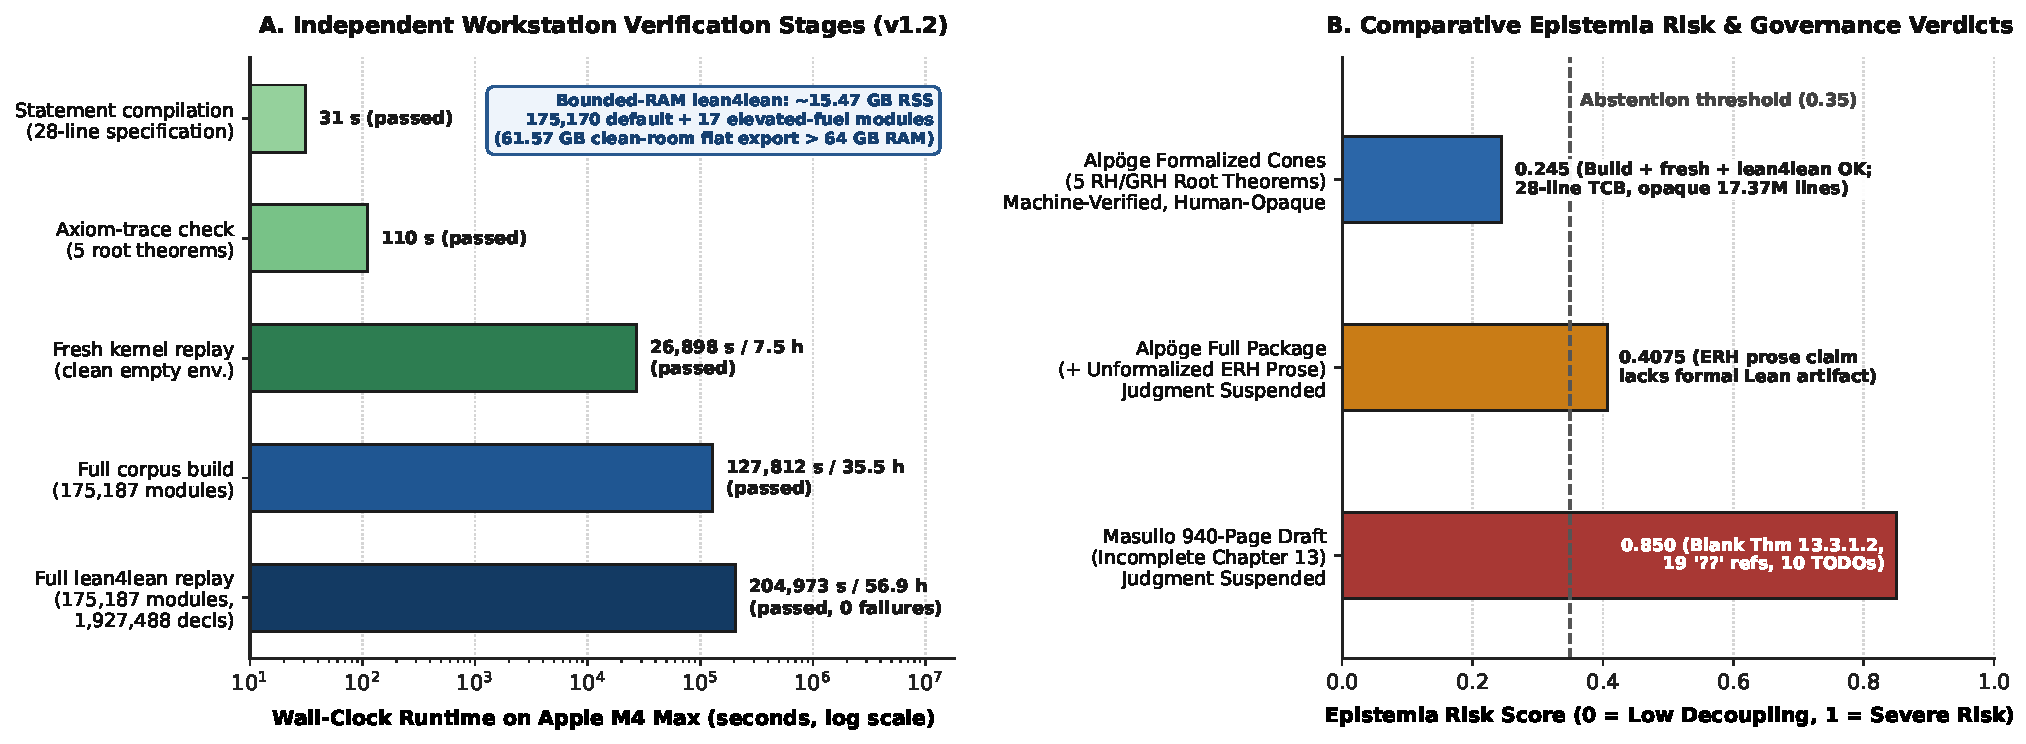
\includegraphics[width=0.98\textwidth,height=0.42\textheight,keepaspectratio]{figures/fig2_verification_and_epistemia.pdf}
  \caption{\textbf{Independent workstation verification stages (v1.1) and comparative Epistemia risk governance.} \textbf{(A)} Wall-clock runtime (log scale) across all four completed Lean~\texttt{v4.33.1} stages on Apple M4 Max (64\,GB unified memory), including transitive fresh-environment replay (26,898\,s, clean exit), alongside the local 46.47\,GB flat-export memory ceiling blocking local external-kernel replay. \textbf{(B)} Normalized Epistemia risk scores across Alp{\"o}ge's five formalized theorems (0.245, machine-verified yet human-opaque), Alp{\"o}ge's full package including unformalized ERH prose (0.4075, judgment suspended), and Masullo's 940-page informal draft (0.850, judgment suspended).}
  \label{fig:verif_epistemia}
\end{figure}

\subsection{Metamathematical Significance of Standard Axiom Closure}

To readers outside type theory, the three-item log \texttt{[propext, Classical.choice, Quot.sound]} may resemble routine compiler output; metamathematically, it settles a foundational question opened by G{\"o}delian incompleteness. Because the Riemann Hypothesis is equivalent to a $\Pi_1^0$ arithmetical sentence---for example, Lagarias's elementary inequality $\sigma(n) \le H_n + e^{H_n}\log H_n$ for all $n \ge 1$~\cite{lagarias2002}---a counterexample would in principle be finitely checkable, leaving open the logical possibility that RH could hold in the standard natural numbers while remaining independent of standard mathematical axioms.

Lean~4's kernel implements dependent type theory augmented solely by three canonical principles: \texttt{propext} (propositional extensionality), \texttt{Classical.choice} (standard classical choice), and \texttt{Quot.sound} (quotient soundness). While this dependent type-theoretic foundation is stronger than elementary Peano Arithmetic (comparable in consistency strength to standard ZFC set theory with universe levels), it is completely standard across modern mathematics. Confirming that all five root theorems discharge strictly over \texttt{[propext, Classical.choice, Quot.sound]} certifies that RH and Dirichlet GRH require \textbf{no exotic large-cardinal hypotheses, no new physical postulates, and no unverified axioms}: their truth is already deductively contained within standard mathematical foundations.

\subsection{Transparent Boundaries, Hardware Limits, and Memory-Bounded Multi-Kernel Escalation}
\label{sec:boundaries}

Scientific honesty requires distinguishing clearly between what \emph{our} independent 64\,GB workstation run has certified end to end, how a memory-bounded execution redesign overcame monolithic export limits, and what residual verification boundaries remain open:
\begin{enumerate}
  \item \textbf{Lean \texttt{v4.33.1} Kernel Replay \& Metaprogramming Clearance (Completed):} Both default checking and full transitive replay (\texttt{lake env leanchecker -{}-fresh}, 26,898\,s, zero exit status) completed cleanly from an empty kernel environment, eliminating \texttt{.olean} corruption, environment-hacking, and metaprogramming bypass risks under Lean~\texttt{v4.33.1}. Because Lean's bundled checker shares Lean's own core kernel implementation, independent external-kernel replay constitutes a distinct verification layer.
  \item \textbf{Flat-Export Memory Wall vs.\ Bounded-RAM Module-by-Module \texttt{lean4lean} Escalation (Active Streaming \& Limitations):} We compiled independent external verification tools (\texttt{nanoda} and Lean's export serializer) against Lean~\texttt{v4.33.1}. Single-threaded flat serialization of the full proof graph (measuring 61,570,595,788 bytes, 61.57\,GB, at full completion) expanded to 46.47\,GB on our 64\,GB host and triggered virtual memory thrashing before completion. To bypass this monolithic memory wall without dropping independent kernel checking, we compiled \texttt{lean4lean} (commit \texttt{67f63b0c}, pinned to Lean~\texttt{v4.33.1})~\cite{carneiro2026} and drove its unmodified import-replay kernel verifier sequentially over exact \texttt{.olean} module lists in 3 parallel workers processing 10-module streaming chunks (with aggressive allocator purging and a $\ge 45\%$ free-memory guard, reserving heavy apex modules for single-worker serial replay). This eliminates both the 61.57\,GB monolithic serialization spike and the prefix-scanning memory spikes of directory-glob invocations (1,671 nested module-name prefix collisions in the archive), holding steady-state combined worker memory around 15.47\,GB (88\% free system memory, zero new swap growth) alongside co-resident production services.
  \begin{itemize}
    \item \textbf{Verified Snapshot (2026-11-24T05:19:45Z):} \textbf{28,357 / 175,187} unique project modules and \textbf{616,173} declarations verified with \textbf{0 failures}: root statements (1/1), auxiliary lemmas (167/167), positivity theory (449/449), ground theory (8,507/8,507), and the entire formalism layer (18,254/18,254), plus initial reciprocity modules (979/3,845). Crucially, 28,352 modules passed under default fuel limits, while the exact \textbf{5 computationally dense kernel-decision modules} (one Chebyshev prime-bound small-loop module verifying 10 declarations in 26,967\,ms, and four dyadic prime-interval modules verifying 2 declarations each in 11,574--11,721\,ms) passed deterministically upon automatic escalation to elevated reduction and recursion fuel limits.
    \item \textbf{Explicit Dual Limitations:} First, our local checkpointed sweep is \textbf{still streaming asynchronously} across the remaining reciprocity, companion, core development (141,928 modules), and serial apex modules; accordingly, full 175,187 / 175,187 local \texttt{lean4lean} closure is \emph{not} claimed until the background sweep exits cleanly. Second, as documented by Carneiro~\cite{carneiro2026}, \texttt{lean4lean} is an external Lean-implemented kernel port derived directly from Lean's C++ kernel architecture (backed by formal metatheory verification and explicit fuel-bounded loops); therefore, unlike clean-room Rust/C reimplementations (\texttt{nanoda}, \texttt{con-leche}), \texttt{lean4lean} provides an independent executable and fuel-audited replay while sharing design lineage with Lean's C++ kernel. Clean-room flat-export replay remains constrained by the 82.6--98.8\,GiB peak host RAM footprint reported externally for 61.57\,GB flat export processing.
  \end{itemize}
  \item \textbf{Parallel Institutional Multi-Kernel Reports (External Context):} Independently of our 64\,GB workstation audit, the Lean FRO and Mathlib Initiative issued a joint verification statement certifying statement fidelity and Lean compilation on November 21, 2026~\cite{leanfro2026}, and Andrew Sutherland (MIT) publicly documented high-memory independent replays using external kernels including \texttt{nanoda}, \texttt{con-leche}, and \texttt{lean4lean}~\cite{sutherland2026}---notably matching word-for-word the exact 5 kernel-decision modules that triggered elevated fuel locally. Those external high-RAM results corroborate clean-room kernel soundness while leaving \textbf{human epistemic comprehension} unresolved.
  \item \textbf{Unformalized Extrapolation to ERH:} While the accompanying prose note anticipates extension to the Extended Riemann Hypothesis (ERH), only RH and Dirichlet GRH are formalized and verified in the root Lean modules.
\end{enumerate}

\section{Deductive Spine Cartography and Six Barrier-Breaking Motifs}

To make the inner logic of 17.37 million lines of code accessible to human mathematicians, we combine a three-step conceptual bridge with full topological mining of the compiled dependency graph (detailed further in our companion mathematical architecture primer):
\begin{itemize}
  \item \textbf{Intuition (Why Classical Tools Stall):} Proving RH reduces via the Guinand--Weil explicit formula to certifying non-negativity of a family of spectral test functionals. Over function fields, Stepanov's auxiliary-polynomial method detects zero multiplicity by taking algebraic derivatives---an operation with no naive analog over $\mathbb{Z}$.
  \item \textbf{Mechanism (Pure Algebraic Architecture, Not Mysticism):} Rather than invoking an exotic physical operator, Alp{\"o}ge's codebase generalizes classical divisibility ideas (Chebyshev/Stepanov) through arithmetic geometry and automorphic forms: it builds iterated chains of unitary \emph{theta lifts} $U(X_0) \to \dots \to U(X_m)$ ($m \sim \sqrt{X}$) to simulate differential multiplicity natively over $\mathbb{Z}$, transforms Gan--Gross--Prasad (GGP) periods into Bessel periods via Rallis's \emph{seesaw} identity, and controls arithmetic heights and denominators via Bost's slope inequality, Siegel mass formulas, and Galois modularity patching.
  \item \textbf{Empirical Footprint in the Lean Dependency Graph:} Topological mining across 818,755 theorems and lemmas reconstructs the exact library stratification (\textbf{Table~\ref{tab:library_strata}} and \textbf{Figure~\ref{fig:spine_arch}}).
\end{itemize}

\begin{table}[!htb]
\centering
\caption{Stratified library architecture of the compiled Lean~4 corpus (175,187 project modules, 818,755 theorems and lemmas, maximum graph depth 43).}
\label{tab:library_strata}
\footnotesize
\setlength{\tabcolsep}{5pt}
\begin{tabular}{@{}lrrcc>{\raggedright\arraybackslash}p{0.34\textwidth}@{}}
\toprule
\textbf{Library Layer} & \textbf{Modules} & \textbf{Thms/Lemmas} & \textbf{Depth} & \textbf{Share} & \textbf{Primary Structural Role} \\
\midrule
Root Specification \& Exports & 5 & 9 & 0--3 & $<$0.01\% & Root exports and Mathlib-anchored targets \\
Core Development Layer & 141,928 & 562,329 & 2--43 & 81.02\% & Abelian/automorphic schemes, Weil bounds, Galois modularity, theta lifts \\
Formalism Layer & 18,254 & 162,118 & 4--43 & 10.42\% & Hermitian curvature, mass formulas, period integrals, Gamma factors \\
Ground Theory Layer & 8,507 & 54,211 & 5--32 & 4.86\% & Local/global fields, Tate thesis, Arakelov heights, $p$-adic Hodge theory \\
Reciprocity Theory Layer & 3,845 & 27,722 & 6--36 & 2.19\% & Reductive groups, birational geometry, toroidal compactification, descent \\
Companion Theory Layer & 2,027 & 9,419 & 5--30 & 1.16\% & Unitary $p$-adic weights, product formulas, Pieri rules \\
Positivity Theory Layer & 449 & 2,702 & 6--13 & 0.26\% & Automorphic positivity functionals and nonvanishing criteria \\
Auxiliary Lemmas \& Build Aids & 172 & 245 & 8--25 & 0.10\% & Shared auxiliary lemmas and inert tactic denylists \\
\bottomrule
\end{tabular}
\end{table}

\begin{figure}[!htb]
  \centering
  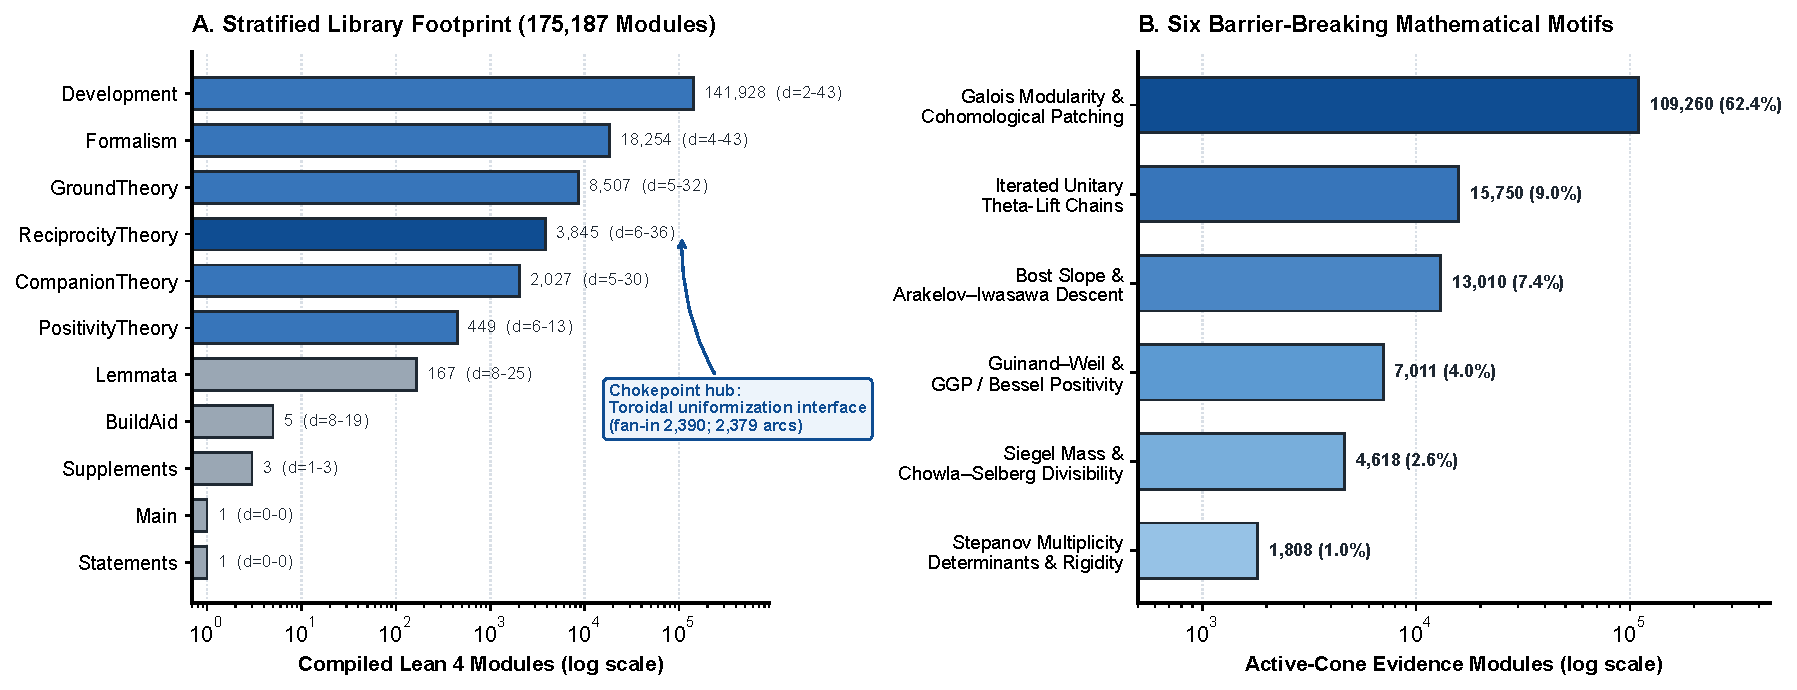
\includegraphics[width=0.98\textwidth,height=0.45\textheight,keepaspectratio]{figures/fig1_epistemic_spine_architecture.pdf}
  \caption{\textbf{Deductive spine cartography of the 175,187-module Lean~4 proof corpus.} \textbf{(A)} Module counts (log scale) and deductive depth spans across all 11 library layers, highlighting the structural chokepoint in the toroidal uniformization interface (depth~6, fan-in~2,390, 2,379 cross-layer arcs). \textbf{(B)} Active-cone module distribution across the six barrier-breaking mathematical motifs identified by empirical clustering.}
  \label{fig:spine_arch}
\end{figure}

Rather than forming an unstructured graph, the dependency cone contracts sharply at \textbf{deductive depths 6--7} inside the reciprocity layer. The top cross-layer pivot is the toroidal uniformization conclusion interface (depth~6, fan-in~2,390, 2,379 cross-layer arcs, 0~theorems), alongside its sister extension-descent uniqueness interface (fan-in~2,284, 2,283 cross-layer arcs). Source inspection shows this hub couples CM-field involutions, group-object ring actions, semiabelian degeneration data, twisted trace-form isomorphisms, and boundary unit criteria, acting as the geometric interface tying foundational schemes to downstream positivity proofs.

Empirical clustering across the active cone quantifies six barrier-breaking mathematical families (\textbf{Figure~\ref{fig:spine_arch}B}):
\begin{enumerate}
  \item \textbf{Galois Modularity \& Cohomological Patching (109,260 modules):} Bypasses elementary-method insufficiency via {\'e}tale/$p$-adic Hodge comparisons, discrete series congruences, and Taylor--Wiles modularity patching.
  \item \textbf{Iterated Unitary Theta-Lift Chains (15,750 modules):} Bypasses contour convexity/parity ceilings by chaining unitary theta lifts $U(X_0) \to \dots \to U(X_m)$ ($m \sim \sqrt{X}$) to simulate differential multiplicity natively over $\mathbb{Z}$.
  \item \textbf{Bost Slope \& Arakelov--Iwasawa Descent (13,010 modules):} Bypasses unbounded height growth via Bost's slope inequality, a Behrend-chosen Iwasawa tower, and weakened Vandiver control with global Artin reciprocity and Hermitian Hasse principles.
  \item \textbf{Guinand--Weil Explicit Formula \& GGP/Bessel Positivity (7,011 modules):} Bypasses local sign-indefiniteness by certifying explicit test functionals $W(\cdot) \ge 0$ via determinants and Rallis \emph{seesaw} Bessel periods.
  \item \textbf{Siegel Mass \& Chowla--Selberg Divisibility (4,618 modules):} Bypasses class-number denominator explosion via unitary Siegel mass formulas and graded Weyl module dominance.
  \item \textbf{Stepanov Multiplicity Determinants \& Rigidity (1,808 modules):} Bypasses pointwise off-line zero bounds using cuspidal strong multiplicity-one rigidity and Gelfand--Kazhdan duality.
\end{enumerate}

\section{Comparative Forensic Evaluation of Formal and Informal Proof Submissions}

While the Lean corpus discharges every dependency syntactically (0~\texttt{sorry}, clean build exit, transitive \texttt{-{}-fresh} replay verified), auditing Masullo's 940-page informal manuscript~\cite{vakil2026} reveals the exact mirror-image failure mode. Although Chapters~1--12 develop Hardy--Sobolev spaces $W_I^{s,2}(G)$, periodic Schauder bases, and quotient stacks toward a trace formula (Theorem~12.5.1.1, p.\,519), structural parsing uncovers \textbf{critical incompleteness in the conclusive chapters}:
\begin{itemize}
  \item In Section~12.4.1 (pp.\,514--515), author footnote~2 leaves a placeholder instruction to revise the $(\lambda, \varepsilon)$-cutoff and re-establish convergence of integral~(12.4.1.23).
  \item \textbf{Chapter~13 (\emph{Zeros of Hecke $L$-functions}, pp.\,521--522)} has empty stub headings for Sections~13.1 and~13.2, references a nonexistent ``Theorem~??'', and leaves the core bridge---\textbf{Theorem~13.3.1.2 (Divisor of $L(s, \chi)$)}---completely empty beneath footnotes ``\emph{2 Insert statement.}'' and ``\emph{3 State and prove the Main Theorems...}''.
  \item Across the 940 pages, forensic indexing located 19 broken \texttt{??} cross-references, 10 author draft TODO notes, and 13 empty/near-empty pages ($<400$ characters). Without rigorous closure of the Montel limit interchange deducing $L'_f / L_f$ holomorphy from the regularized trace formula, the informal proof remains analytically open (an unverified prose claim with Epistemia risk 0.850, warranting suspended judgment; \textbf{Figure~\ref{fig:verif_epistemia}B}).
\end{itemize}

\section{Epistemic Governance, Understanding Versus Certification, and the Distillation Horizon}

Evaluated through Quattrociocchi, Capraro, and Perc~\cite{quattrociocchi2025}, William Thurston's classic essay \emph{On Proof and Progress in Mathematics}~\cite{thurston1994}, and Griffiths's resource-rational cognitive science~\cite{griffiths2026}, these results expose two complementary epistemic regimes:
\begin{itemize}
  \item \textbf{Machine-Without-Comprehension (Machine-Verified, Human-Opaque; Epistemia risk 0.245):} Alp{\"o}ge's five formalized RH/GRH theorems clear Lean~\texttt{v4.33.1} compilation and transitive \texttt{-{}-fresh} replay on a minimal 28-line specification (ratio $1.62 \times 10^{-6}$), yet 17.37 million lines of formal tactics vastly exceed bounded human verification budgets. Evaluated as a full package including unformalized ERH prose expectations, epistemic governance suspends judgment (Epistemia risk 0.4075).
  \item \textbf{Intuition-Without-Convergence (Judgment Suspended; Epistemia risk 0.850):} Masullo's manuscript provides human-surveyable prose intuition while lacking conclusive theorem proofs in Chapter~13.
\end{itemize}

As Thurston~\cite{thurston1994} argued three decades before AI-scale theorem proving, mathematics does not advance merely by accumulating certified truth values; it advances through \textbf{human understanding}---compact mental schemas that explain \emph{why} a result holds and transfer across problems. In Griffiths's Marr-level framework~\cite{griffiths2026}, bounded biological minds operate under strict resource-rational constraints, reasoning over compressed conceptual abstractions (such as the six algebraic motifs and the toroidal uniformization hub) rather than millions of micro-rewrites.

Consequently, verifying a 17.37-million-line formal proof completes only \textbf{Phase~1 (Certification)} of mathematical progress. \textbf{Phase~2 (Cognitive Distillation)}---compressing millions of machine-verified lines into transparent, human-surveyable expositions---has immediately emerged as the defining challenge of the field, reflected both in early community prose-reconstruction drafts (such as preliminary third-party prose-reconstruction guides circulated by Michael Rubinstein, Jimmie Adriazola, and Robin Zhang) and in automated structural cartography. By pairing bit-exact kernel certification with stratified dependency spine extraction, interactive dependency navigation, a progressive mathematical primer, and explicit contestability criteria (naming the weakest pivot, executed refutation checks, and empirical revocation conditions), our framework provides reproducible empirical scaffolding for turning machine-verified yet opaque artifacts into genuine human comprehension.

\subsection{Methodological Lessons for Automated Scientific Auditing Systems}

Conducting this end-to-end audit also exposed four structural failure modes in AI-assisted mathematical evaluation, yielding four reusable safeguards directly integrated into CoResearcher:
\begin{enumerate}
  \item \textbf{Artifact-Bound Manuscript Provenance Gating:} When generative models draft technical summaries around complex computational outputs, unconstrained text generation risks fabricating hardware parameters, distorting declaration counts, or inverting comparative epistemic indices. Enforcing deterministic provenance checks that bind every reported metric, SHA-256 digest, and entity-risk ordering strictly to signed JSON and raw log certificates blocks unanchored claims prior to dissemination.
  \item \textbf{Automated Public Dossier Integrity and Hygiene Sealing:} Publishing reproducible scientific evidence alongside proprietary orchestration code requires a deterministic boundary firewall: excluding internal source code, local environment paths, and private internal identifiers while automatically generating checksum manifests, enforcing citation/heading hygiene, and verifying live \texttt{HTTP 200 OK} reachability across external links.
  \item \textbf{Memory-Aware Multi-Kernel Escalation Routing:} Naive escalation from Lean compilation to monolithic flat export (61.57\,GB) fails deterministically via memory exhaustion on 64\,GB workstations. Resource-rational verification planners must estimate serialized export pressure from active module counts and available RAM---routing workstations below clean-room replay headroom ($\sim$82.6--98.8\,GiB+) to memory-bounded module-by-module \texttt{.olean} replay (\texttt{lean4lean} with automatic elevated-fuel retries), while reserving flat-export clean-room kernels (\texttt{nanoda}, \texttt{con-leche}) for high-memory cluster nodes.
  \item \textbf{Deductive Chapter-Bridge Auditing and Barrier-Motif Feedback:} Both informal manuscripts and AI discovery loops benefit from structural closure telemetry: verifying whether named theorems proved in intermediate sections (Theorem~12.5.1.1) connect deductively into conclusive chapters rather than terminating in broken \texttt{??} stubs, and feeding recurring barrier-breaking proof motifs mined from verified dependency cones back into early problem-formulation guidance whenever classical obstructions arise.
\end{enumerate}

\section{Data, Code Availability, and AI Transparency Disclosure}

\paragraph{Data and Code Availability.} All primary cryptographic digests, reference hardware compilation records, raw axiom-trace (SHA-256 \texttt{590d5252...}), transitive fresh-replay (SHA-256 \texttt{ff8ea3d0...}), and bounded-RAM \texttt{lean4lean} module-replay checkpoint telemetry (28,357 / 175,187 modules, 616,173 declarations checked, 0 failures at 2026-11-24T05:19:45Z), along with static soundness counts, stratified dependency spine summaries, interactive dependency explorer, progressive mathematical primer, and comparative forensic inventories for both targets are openly archived in the public verification dossier at \url{https://github.com/Fundacion-de-Neurociencias/riemann-hypothesis-audit-dossier} (v1.1 baseline release tag: \url{https://github.com/Fundacion-de-Neurociencias/riemann-hypothesis-audit-dossier/releases/tag/v1.1}). Automated multi-stage verification is coordinated through CoResearcher~\cite{menendez2026coresearcher} at \url{https://github.com/Fundacion-de-Neurociencias/coresearcher}. All cited repositories are publicly accessible without authentication.

\paragraph{Artificial Intelligence Disclosure.} Autonomous computational orchestration (Lean~4 build supervision, cryptographic checksum verification, bounded-RAM module-by-module kernel replay orchestration, dependency-graph extraction, and PDF structural parsing) was executed via CoResearcher~\cite{menendez2026coresearcher}, and generative AI assistants were employed for editorial polishing and \LaTeX{} typesetting. All empirical measurements were extracted verbatim from deterministic execution logs on local hardware and bound programmatically against immutable JSON certificates, all bibliographic citations and external URLs were independently verified, and the author holds full epistemic and intellectual responsibility for all content.

\bibliographystyle{unsrt}
\bibliography{references}

\end{document}
